\documentclass[a4paper,12pt]{extarticle}
\usepackage[utf8x]{inputenc}
\usepackage[T1,T2A]{fontenc}
\usepackage[russian]{babel}
\usepackage{hyperref}
\usepackage{indentfirst}
\usepackage{listings}
\usepackage{color}
\usepackage{here}
\usepackage{array}
\usepackage{multirow}
\usepackage{graphicx}

\usepackage{caption}
\renewcommand{\lstlistingname}{Программа} % заголовок листингов кода

\bibliographystyle{ugost2008ls}

\usepackage{listings}
\lstset{ %
extendedchars=\true,
keepspaces=true,
language=C,						% choose the language of the code
basicstyle=\footnotesize,		% the size of the fonts that are used for the code
numbers=left,					% where to put the line-numbers
numberstyle=\footnotesize,		% the size of the fonts that are used for the line-numbers
stepnumber=1,					% the step between two line-numbers. If it is 1 each line will be numbered
numbersep=5pt,					% how far the line-numbers are from the code
backgroundcolor=\color{white},	% choose the background color. You must add \usepackage{color}
showspaces=false				% show spaces adding particular underscores
showstringspaces=false,			% underline spaces within strings
showtabs=false,					% show tabs within strings adding particular underscores
frame=single,           		% adds a frame around the code
tabsize=2,						% sets default tabsize to 2 spaces
captionpos=t,					% sets the caption-position to top
breaklines=true,				% sets automatic line breaking
breakatwhitespace=false,		% sets if automatic breaks should only happen at whitespace
escapeinside={\%*}{*)},			% if you want to add a comment within your code
postbreak=\raisebox{0ex}[0ex][0ex]{\ensuremath{\color{red}\hookrightarrow\space}},
texcl=true,
inputpath=listings,                     % директория с листингами
}

\usepackage[left=2cm,right=2cm,
top=2cm,bottom=2cm,bindingoffset=0cm]{geometry}

%% Нумерация картинок по секциям
\usepackage{chngcntr}
\counterwithin{figure}{section}
\counterwithin{table}{section}

%%Точки нумерации заголовков
\usepackage{titlesec}
\titlelabel{\thetitle.\quad}
\usepackage[dotinlabels]{titletoc}

%% Оформления подписи рисунка
\addto\captionsrussian{\renewcommand{\figurename}{Рисунок}}
\captionsetup[figure]{labelsep = period}

%% Подпись таблицы
\DeclareCaptionFormat{hfillstart}{\hfill#1#2#3\par}
\captionsetup[table]{format=hfillstart,labelsep=newline,justification=centering,skip=-10pt,textfont=bf}

%% Путь к каталогу с рисунками
\graphicspath{{fig/}}


\begin{document}	% начало документа

% Титульная страница
\begin{titlepage}	% начало титульной страницы

	\begin{center}		% выравнивание по центру

		\large Санкт-Петербургский Политехнический Университет Петра Великого\\
		\large Институт компьютерных наук и технологий \\
		\large Кафедра компьютерных систем и программных технологий\\[6cm]
		% название института, затем отступ 6см
		
		\huge Сети и телекоммуникации\\[0.5cm] % название работы, затем отступ 0,5см
		\large Отчет по лабораторной работе\\[0.1cm]
		\large Программирование сокетов протоколов TCP и UDP\\[5cm]

	\end{center}


	\begin{flushright} % выравнивание по правому краю
		\begin{minipage}{0.25\textwidth} % врезка в половину ширины текста
			\begin{flushleft} % выровнять её содержимое по левому краю

				\large\textbf{Работу выполнил:}\\
				\large Ерниязов Т.Е.\\
				\large {Группа:} 43501/3\\
				
				\large \textbf{Преподаватель:}\\
				\large Алексюк А.О.

			\end{flushleft}
		\end{minipage}
	\end{flushright}
	
	\vfill % заполнить всё доступное ниже пространство

	\begin{center}
	\large Санкт-Петербург\\
	\large \the\year % вывести дату
	\end{center} % закончить выравнивание по центру

\thispagestyle{empty} % не нумеровать страницу
\end{titlepage} % конец титульной страницы

\vfill % заполнить всё доступное ниже пространство



\section{Цель работы}

Изучение принципов программирования сокетов протоколов TCP и UDP.

\section{Программа работы}

\begin{itemize}
\item разработать простейший клиент и сервер на основе протоколов TCP и UDP
\item разработать прикладной протокол в соответствии с индивидуальным заданием, реализовать протокол в виде клиент-серверного приложения на основе протоколов TCP и UDP
\item выполнить дополнительное задание
\end{itemize}

\section{Ход выполнения работы}

\subsection{Простейшие клиент и сервер}
Простейшие клиент и сервер были выполнены на основе протоколов TCP и UDP, а также адаптированы под ОС Windows и Linux. Сервер выполняет функции эхо-сервера, т.е. принимает сообщения от клиентов и посылает копии обратно. Клиент посылает сообщение, после чего завершается.

\subsection{Индивидуальное задание}

В качестве индивидуального задания была выбрана система торгов. На торги выставляются лоты, имеющие начальную стоимость. Участники торгов могут повышать стоимость лота. Распорядитель может прекратить торги. При окончании торгов всем участникам рассылаются результаты торгов.

Серверное приложение реализует следующие функции:
\begin{itemize}
\item Прослушивание определенного порта
\item Обработка запросов на подключение по этому порту от клиентов системы торгов (как распорядитель или участник торгов)
\item Поддержка одновременной работы нескольких клиентов системы
торгов через механизм нитей
\item От участников торгов: прием запросов на передачу списка лотов
\item От участников торгов: прием запросов на повышение стоимости лота
\item От распорядителя: прием запроса на добавление нового лота с первоначальной стоимостью
\item От распорядителя: прием запроса об окончании торгов
\item Осуществление добавления лота, учет повышения стоимости лота участниками, завершение торгов и рассылка результатов торгов всем участникам
\item Обработка запроса на отключение клиента
\item Принудительное отключение клиента
\end{itemize}

Клиентское приложение реализует следующие функции:

\begin{itemize}
\item Установление соединения с сервером
\item Регистрация в качестве распорядителя или участника
\item Участник: передача запроса о выводе списка лотов
\item Участник: передача запроса о повышении стоимости лота
\item Распорядитель: передача запроса о добавлении лота
\item Распорядитель: передача запроса о прекращении торгов
\item Получение результатов торгов от сервера
\item Разрыв соединения
\item Обработка ситуации отключения клиента сервером
\end{itemize}


\subsubsection{Реализация на TCP}

Для реализации данной системы был разработан текстовый асинхронный протокол. Максимальная длина сообщения 1000 символов. 


\paragraph{Описание протокола:}

Сообщение клиента всегда содержит команду, определяющее тип сообщения. Некоторые типы сообщений содержат также поле опций. В конце каждого сообщения ставится символ $\backslash$n.

Поле команды имеет размер до 5 байт. Поле опций может (в зависимости от команды) отсутствовать или содержать до 2 частей. Опции и команды разделяются пробелом.

\begin{itemize}
\item Команда для начала сеанса - new. Опций нет.
\item Команда для авторизации - login. Опции - имя пользователя.
\item Команда для получения списка лотов - 1. Опций нет.
\item Команда для повышения ставки - bet. Опции - наименование лота, ставка.
\item Команда для получения указаний по созданию нового лота - 2. Опций нет. 
\item Команда для создания нового лота - lot. Опции - наименование лота, начальная ставка. 
\item Команда для просмотра онлайн пользоватей - 3. Опций нет.
\item Команда на отключение от сервера - 4. Опций нет.
\item Команда для окончания торгов - 5. Опций нет.
\end{itemize}


Сообщения сервера также всегда заканчиваются символом $\backslash$n. Cообщения не требуют специальной обработки и просто выводятся пользователю.

\paragraph{Описание программы:}

Сервер имеет 1 слушающий порт, по которому принимает от клиентов запросы на соединение. При подсоединении очередного клиента, для связи с ним выделяется отдельный сокет, прием из которого осуществляется в отдельном потоке. 

После подключения клиента сервер ожидает команды для авторизации нового пользователя. Остальные команды в этот момент для клиента недоступны. После авторизации сервер записывает его сокет, имя пользователя и информацию о типе клиента (распорядитель или участник).

Обработчик, в зависимости от соответствующего типа команды, формирует ответное сообщение пользователю.

Для управления сервером предусмотрен поток для опроса стандартного потока ввода. Его работа схожа с работой потока приема сообщений от пользователя. При вводе команды вызывается обработчик. 

У клиента создаются два потока для отправки сообщений и принятия сообщений от сервера в асинхронном режиме. 

\subsubsection{Реализация на UDP}

\paragraph{Описание протокола:}

Реализация прикладного протокола на UDP схожа с реализацией на TCP. Протокол отличается тем, что теперь после авторизации пользователя в начале сообщения передается id пользоватедя. Также теперь нельзя посмотреть онлайн-пользоватей. Максимальное количество пользователей - 10, так как для id зарезервирован всего 1 байт.

После отпраки команды на авторизацию клиент принимает сообщения от сервера с выделенным id для этого клиента. Это сообщение имеет длину 3 байта, последний байт и есть id клиента.

\paragraph{Описание программы:}

В отличие от варианта TCP, здесь не происходит установления соединения и все сообщения передаются через один сокет. Для каждого клиента больше не создается новый поток, поэтому при авторизации пользователя сервер отсылает клиенту его id, который клиент потом использует для его идентификации.

\subsection{Дополнительное задание}

В качестве дополнительного задания необходимо исследовать реальные прикладные протоколы. Необходимо "притвориться" клиентом и подключиться к одному из существующих общедоступных серверов.

В качестве утилиты для подключения к серверам была выбрана telnet.

\subsubsection{Подключение к веб-серверу и запрос веб-страницы}

Был произведен запрос веб-страницы с сервера tiger.ftk.spbstu.ru (рис. 3.2) Подключение производится по используемому протоколом HTTP порту 80. Сервер вернул код 200 в заголовке ответа, что говорит об успешной обработке запроса.

\begin{figure}[H]
	\begin{center}
		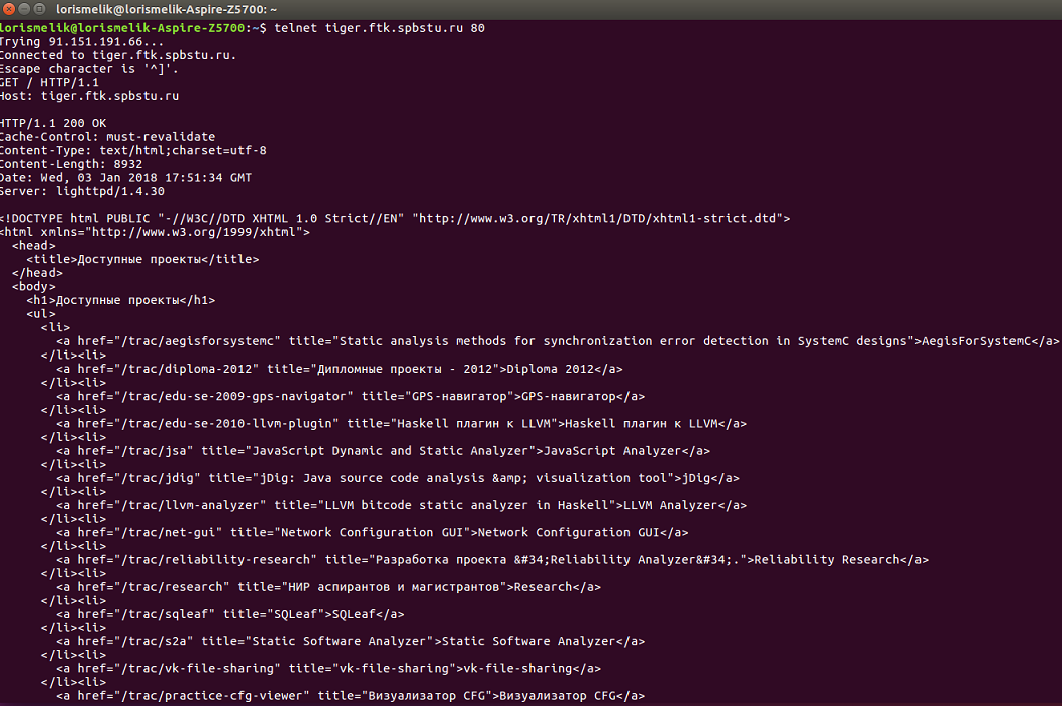
\includegraphics[scale=0.7]{http}
		\caption{Запрос веб-страницы} 
		\label{pic:pic_name} % название для ссылок внутри кода
	\end{center}
\end{figure}

\subsubsection{Загрузка файла с ftp-сервера}

Протокол FTP использует 2 соединения - для передачи команд и для передачи данных. Поэтому подключение к нему производится в 2 этапа: сначала производится подключение к порту 21 (для передачи команд) и авторизация, затем переход в пассивный режим и подключение из другого терминала к порту, указанному сервером 
\begin{figure}[H]
	\begin{center}
		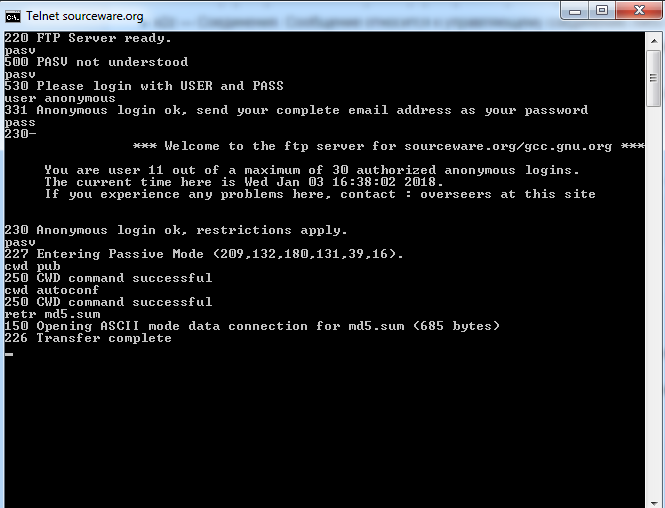
\includegraphics[scale=0.7]{ftp0}
		\caption{Загрузка файла с FTP-сервера} 
		\label{pic:pic_name} % название для ссылок внутри кода
	\end{center}
\end{figure}

Подключаемся по адресу выданному сервером: 209.132.180.39.16:10000

\begin{figure}[H]
	\begin{center}
		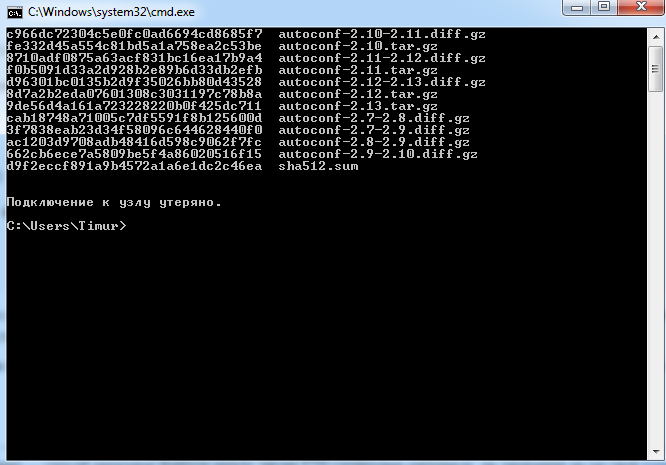
\includegraphics[scale=0.7]{ftp1}
		\caption{Загрузка файла с FTP-сервера} 
		\label{pic:pic_name} % название для ссылок внутри кода
	\end{center}
\end{figure}

\subsubsection{Отправка письма на SMTP-сервер}

Попытаемся авторизоваться на SMTP-сервере yandex с использованием TLS для защищенной передачи данных.


\begin{figure}[H]
	\begin{center}
		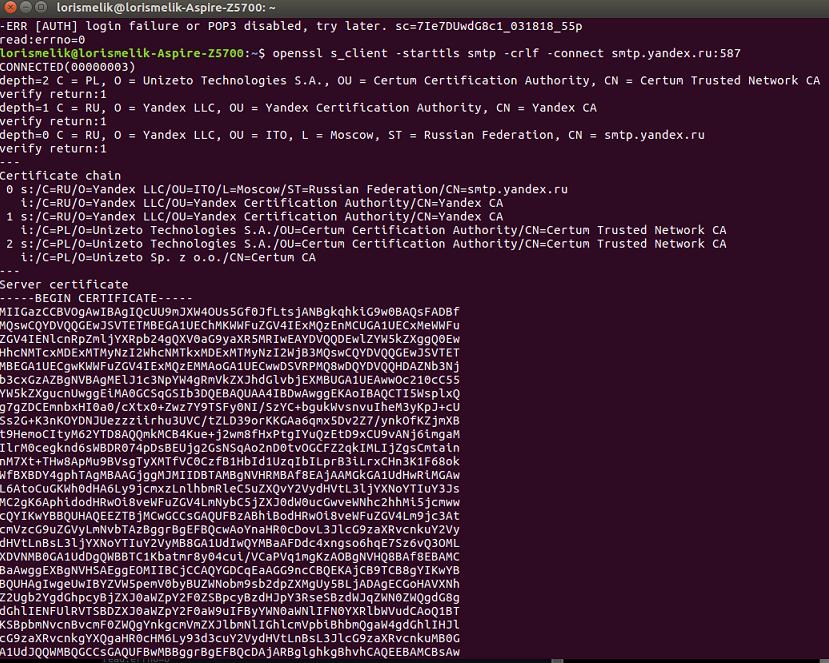
\includegraphics[scale=0.7]{smtp0}
		\caption{Отправка письма на SMTP-сервер через TLS-подключение}
		\label{pic:pic_name} % название для ссылок внутри кода
	\end{center}
\end{figure}

\begin{figure}[H]
	\begin{center}
		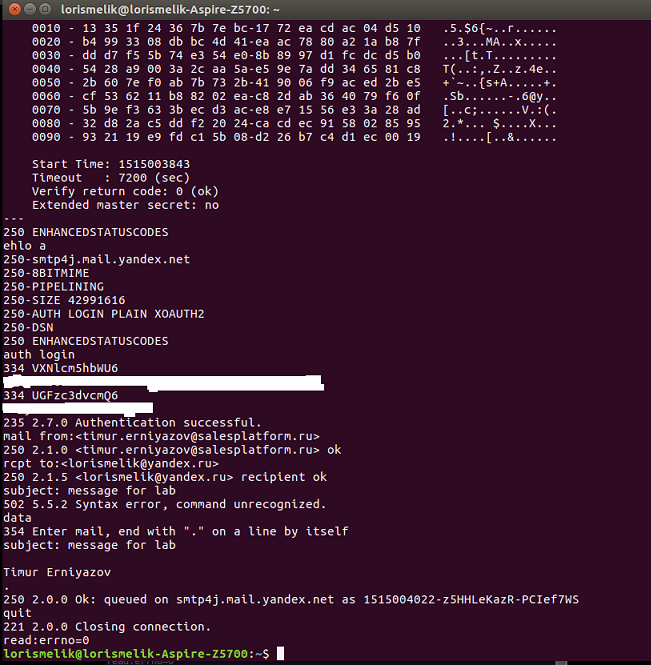
\includegraphics[scale=0.7]{smtp1}
		\caption{Отправка письма на SMTP-сервер через TLS-подключение}
		\label{pic:pic_name} % название для ссылок внутри кода
	\end{center}
\end{figure}



\subsubsection{Получение письма с POP3-сервера}

Проверим почту и получим письмо 

\begin{figure}[H]
	\begin{center}
		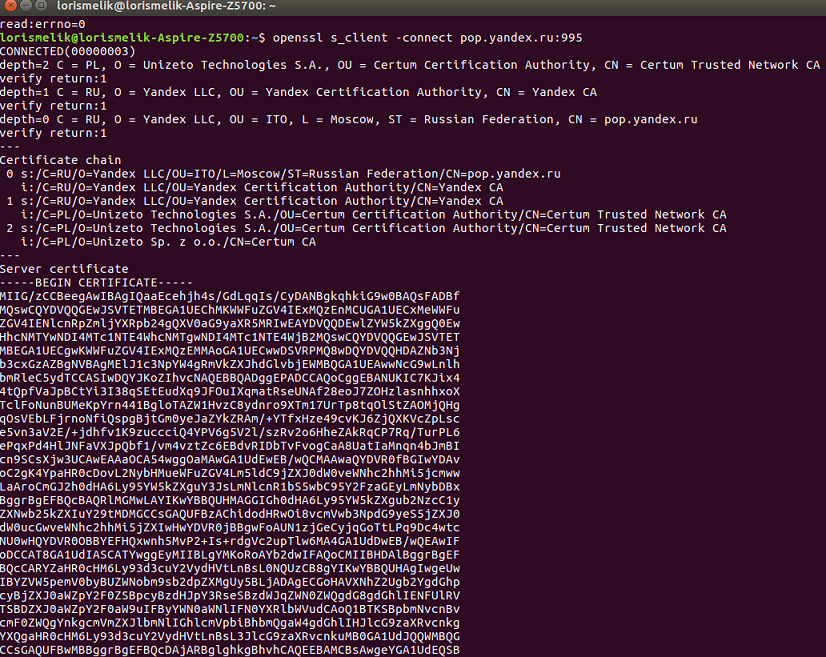
\includegraphics[scale=0.7]{pop3_1}
		\caption{POP3} 
		\label{pic:pic_name} % название для ссылок внутри кода
	\end{center}
\end{figure}

\begin{figure}[H]
	\begin{center}
		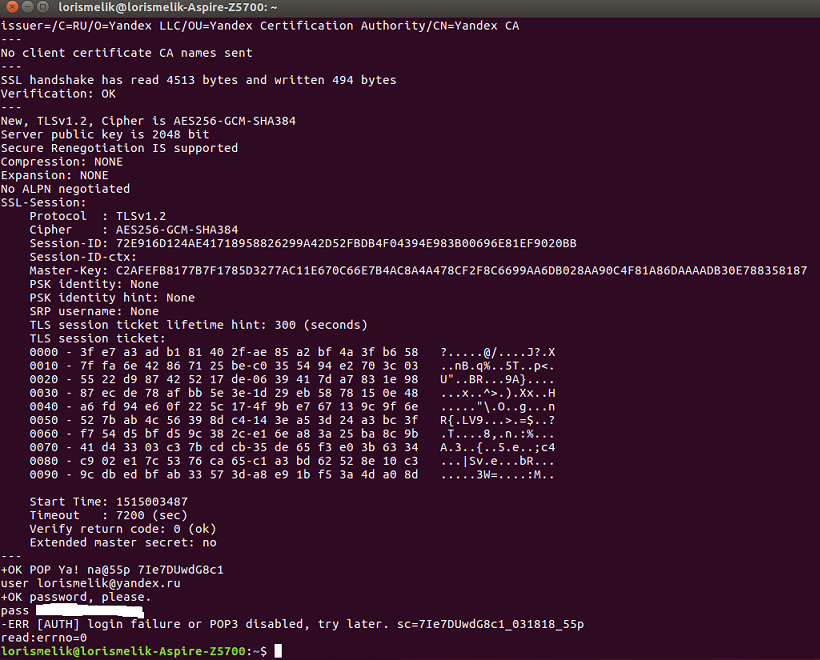
\includegraphics[scale=0.7]{pop3_2}
		\caption{POP3} 
		\label{pic:pic_name} % название для ссылок внутри кода
	\end{center}
\end{figure}

Yandex отключил поддержку pop3 протокола, поэтому проверить почту не удалось.


\section{Выводы}

В ходе работы был разработан и реализован в виде приложения прикладной протокол. В результате этого были изучены принципы программирования сокетов TCP и UDP. Основной проблемой при реализации приложения на TCP была необходимость контроля длины посылки. Ее решением стало добавление символа окончания посылки. TCP требует установления соединения, поэтому на сервере выделяется поток, в котором происходит прием запросов на соединение от клиентов через выделенный для этого сокет. После подключения очередного клиента порождается отдельный поток, осуществляющий обмен пакетами с этим клиентом через отдельный сокет. 

В реализации на UDP сервер обменивается пакетами со всеми клиентами в одном потоке и через один сокет, т.к. нет установления соединения. Для идентификации пользователей в сообщение добавилось поле id.

Также были исследованы прикладные протоколы. Как выяснилось, почтовые сервера могут требовать обязательного использования защищенного подключения.

\end{document}
